\documentclass[11pt,a4paper]{article}
\usepackage[utf8]{inputenc}
\usepackage[T1]{fontenc}
\usepackage{lmodern}
\usepackage[margin=25mm,headsep=8mm,footskip=12mm]{geometry}
\usepackage{amsmath,amssymb,mathtools,amsthm}
\usepackage{microtype,booktabs,array,longtable,graphicx,xcolor,enumitem}
\usepackage{tikz}
\usetikzlibrary{arrows.meta,positioning,calc,fit}
\usepackage[font=small,labelfont=bf]{caption}
\usepackage{fancyhdr}
\usepackage[unicode,pdfencoding=auto]{hyperref}
\definecolor{ReportNavy}{HTML}{17324D}
\definecolor{ReportTeal}{HTML}{176B78}
\hypersetup{colorlinks=true,linkcolor=ReportNavy,urlcolor=ReportTeal,
  pdfauthor={},pdftitle={Initial purity in quantum learning without resets},
  pdfsubject={A self-contained explanatory report},pdfkeywords={},
  pdfcreator={pdfLaTeX}}
\setlength{\headheight}{14pt}
\pagestyle{fancy}
\fancyhf{}
\fancyhead[L]{\small Learning without resets}
\fancyhead[R]{\small Explanatory report}
\fancyfoot[C]{\small\thepage}
\renewcommand{\headrulewidth}{0.25pt}
\setlength{\parindent}{1.2em}
\setlength{\parskip}{0.25em}
\setlength{\emergencystretch}{2em}
\linespread{1.06}
\setlist{topsep=4pt,itemsep=3pt,parsep=1pt}
\clubpenalty=10000
\widowpenalty=10000
\displaywidowpenalty=10000
\raggedbottom
\allowdisplaybreaks[1]
\numberwithin{equation}{section}
\newtheorem{theorem}{Theorem}[section]
\newtheorem{lemma}[theorem]{Lemma}
\newtheorem{proposition}[theorem]{Proposition}
\newtheorem{corollary}[theorem]{Corollary}
\theoremstyle{definition}
\newtheorem{definition}[theorem]{Definition}
\newtheorem{example}[theorem]{Example}
\theoremstyle{remark}
\newtheorem*{remark}{Remark}
\DeclareMathOperator{\Tr}{Tr}
\DeclareMathOperator{\rank}{rank}
\DeclareMathOperator{\supp}{supp}
\DeclareMathOperator{\diag}{diag}
\newcommand{\Id}{\mathrm{id}}
\newcommand{\Dep}{\mathcal D}
\newcommand{\EE}{\mathbb E}
\newcommand{\cE}{\mathcal E}
\newcommand{\cD}{\mathcal D}
\newcommand{\norm}[1]{\left\lVert#1\right\rVert}
\newcommand{\abs}[1]{\left\lvert#1\right\rvert}
\newcommand{\ket}[1]{\lvert#1\rangle}
\newcommand{\bra}[1]{\langle#1\rvert}
\newcommand{\braket}[2]{\langle#1\vert#2\rangle}
\newcommand{\JointBudgetFigure}{%
\begin{figure}[htbp]
\centering
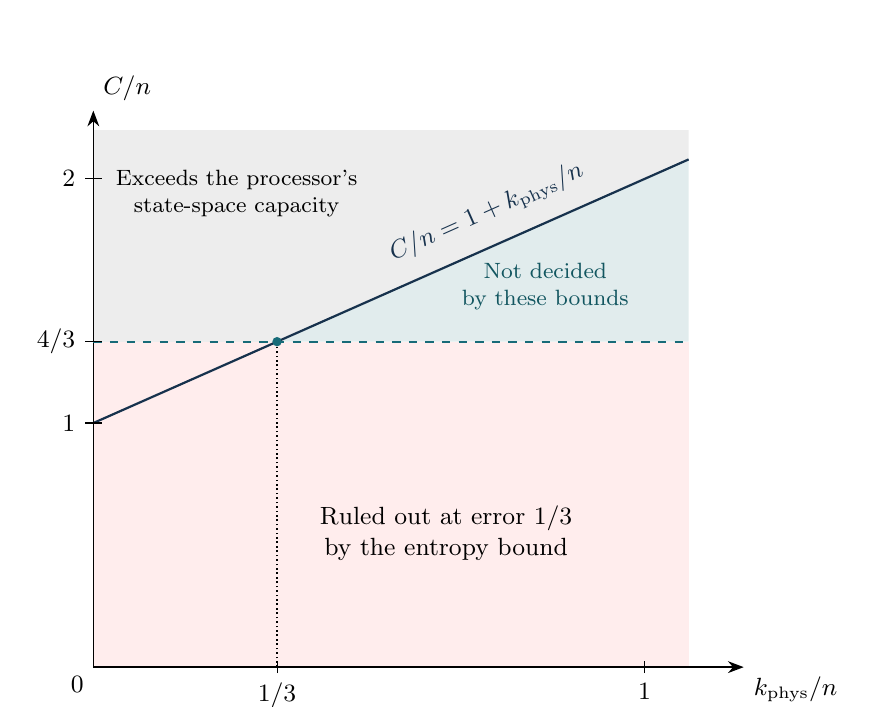
\begin{tikzpicture}[x=7cm,y=3.1cm,font=\small,>=Stealth]
  \fill[black!7] (0,1) -- (1.08,2.08) -- (1.08,2.2) -- (0,2.2) -- cycle;
  \fill[red!7] (0,0) rectangle (1.08,1.333333333);
  \fill[ReportTeal!13] (0.333333333,1.333333333) -- (1.08,1.333333333)
       -- (1.08,2.08) -- cycle;
  \draw[->,semithick] (0,0) -- (1.18,0) node[below right] {$k_{\rm phys}/n$};
  \draw[->,semithick] (0,0) -- (0,2.28) node[above right] {$C/n$};
  \draw[ReportNavy,thick] (0,1) -- (1.08,2.08);
  \node[ReportNavy,rotate=24,above] at (0.73,1.78)
       {$C/n=1+k_{\rm phys}/n$};
  \draw[ReportTeal,thick,dashed] (0,1.333333333) -- (1.08,1.333333333);
  \draw[densely dotted,semithick] (0.333333333,0) -- (0.333333333,1.333333333);
  \fill[ReportTeal] (0.333333333,1.333333333) circle (1.7pt);
  \node[align=center] at (0.64,0.55)
       {Ruled out at error $1/3$\\by the entropy bound};
  \node[align=center,ReportTeal!80!black,font=\footnotesize] at (0.82,1.56)
       {Not decided\\by these bounds};
  \node[align=center,font=\footnotesize] at (0.26,1.94)
       {Exceeds the processor's\\state-space capacity};
  \foreach \y/\lab in {1/1,1.333333333/{4/3},2/2}
    {\draw (-0.015,\y) -- (0.015,\y); \node[left] at (-0.015,\y) {$\lab$};}
  \foreach \x/\lab in {0.333333333/{1/3},1/1}
    {\draw (\x,-0.025) -- (\x,0.025); \node[below] at (\x,-0.025) {$\lab$};}
  \node[below left] at (0,0) {$0$};
\end{tikzpicture}
\caption{Necessary budgets for the weight-one, attenuation-$1/2$ task.
The whole processor has $n+k_{\rm phys}$ qubits, including every retained
record. The entropy condition $C\ge4n/3$ and dimension ceiling
$C\le n+k_{\rm phys}$ meet at $k_{\rm phys}=n/3$.
The teal region merely survives both inequalities; attainability there is
not established. This is not a diagram for a coherent-width convention
that exempts a classical history.}
\label{fig:joint-budget}
\end{figure}%
}
\begin{document}
\thispagestyle{plain}
\begin{center}
  {\color{ReportNavy}\LARGE\bfseries Initial purity in quantum learning without resets\par}
  \vspace{0.5em}
  {\small Explanatory report}
\end{center}
\vspace{0.25em}
\noindent{\color{ReportTeal}\rule{\textwidth}{0.6pt}}
\vspace{0.3em}

\section{One initialized experiment, many possible directions}

A noisy device may preserve a weak correlation even when it destroys almost
everything else. Repeated use of the device then seems to offer a natural
strategy: move a little information into memory, interrogate the device again,
and continue until the accumulated evidence becomes readable. This report asks
when that strategy can work if the entire experiment receives its supply of
initialization only once.

The final answer is just one bit: is the device completely depolarizing, or does
it retain one unknown Pauli correlation? A single initially pure output qubit
could hold that bit. The difficulty is therefore not the size of the answer.
It is the need to discover a direction that is hidden among many possible
operator directions, while every operation and every retained record must fit
within a processor whose initial purity is fixed.

Two results make this distinction quantitative. The decision signal is the
largest difference in one outcome's probability between the null and the
uniform alternative mixture. For the full family of $M=4^n-1$ nonidentity
Pauli directions, the largest attainable signal from one clean qubit,
optimized over all finite query budgets, has scale
\[
 \min\left\{1,\frac{\lambda}{M(1-\lambda)}\right\},
 \qquad 0\leq\lambda<1.
\]
Here $\lambda$ is the coefficient retained by the hidden mode. At fixed
$0<\lambda<1$, the signal is exponentially small in the number $n$ of queried
qubits, however long the initialized experiment runs. Close to exact
conservation, a finite pointer scan achieves the same scale up to universal
constants.

A second result concerns the much smaller family of $3n$ weight-one directions.
At $\lambda=1/2$, constant-error detection still requires a linear initial
entropy deficit. In particular, error at most $1/3$ requires at least $4n/3$
bits of this resource. For a product of clean and maximally mixed qubits, the
entropy deficit is exactly the number of initially clean qubits.

The companion report, \emph{Coherent memory in Pauli channel learning}, asks how
many coherent reference qubits are needed when fresh probes and classical
records are available throughout the experiment. The weight-one comparison
below shows why that access model and a fixed initialization supply have
different limits.

\section{The channel and the complete processor}

\subsection{States, Pauli coefficients, and a physical promise}

A register with a $d$-dimensional state space is described by a density operator
$\rho$: a positive semidefinite $d\times d$ matrix with $\Tr\rho=1$. A pure state
has the form $|\psi\rangle\langle\psi|$; the maximally mixed state is $I/d$.
The trace $\Tr B$ is the sum of the diagonal entries of $B$.
An observable is a Hermitian operator $P$, and its measured mean in state
$\rho$ is $\Tr(P\rho)$.
The symbol $I$ denotes the identity operator on the register indicated by its
context.

The queried register $S$ contains $n\geq1$ qubits, so $d=2^n$. The Hermitian
Pauli strings $P_0=I,P_1,\ldots,P_M$, where $M=d^2-1$, form an orthogonal basis
for its operators:
\begin{equation}
 \Tr(P_aP_b)=d\,\mathbf 1_{\{a=b\}}.
 \label{q:pauli-orthogonal}
\end{equation}
Each string is a tensor product of the one-qubit observables $I,X,Y,Z$.
A qubit has a two-dimensional state space with orthonormal basis
$|0\rangle,|1\rangle$. In that basis the three matrices are
\[
 X=\begin{pmatrix}0&1\\1&0\end{pmatrix},\qquad
 Y=\begin{pmatrix}0&-i\\i&0\end{pmatrix},\qquad
 Z=\begin{pmatrix}1&0\\0&-1\end{pmatrix},
\]
where $i^2=-1$. Each is Hermitian and squares to the identity. A nonidentity
Pauli string likewise satisfies $P_a^2=I$ and has observable outcomes
$+1$ and $-1$. Its support is the set of sites with a nonidentity factor;
its weight is the number of those sites. For instance,
$X\otimes I\otimes Z$ has support $\{1,3\}$ and weight two.
The number of nonidentity strings is $4^n-1$, rather than $2^n-1$, because
operators form a $d^2$-dimensional vector space. The coefficient of $P_a$ in a
state describes an observable correlation, not a state eigenvalue.

The device is promised to be either
\begin{align}
 \mathcal D(B)&=\frac{I}{d}\Tr B, \label{q:null-channel}\\
 \mathcal E_{a,\lambda}(B)
   &=\frac{I\Tr B+\lambda P_a\Tr(P_aB)}{d},
   \quad a\in\{1,\ldots,M\},\quad 0\leq\lambda\leq1 .
 \label{q:spike-channel}
\end{align}
Here $B$ is an arbitrary input operator. The label $a$ is unknown and remains
fixed throughout the run. The parameter $\lambda$ is dimensionless. It
multiplies the expectation of $P_a$ and all other nonidentity Pauli expectations
are erased. The constructive procedures below know $\lambda$; the upper bounds
on information remain valid even when it is known.

These formulas define ordinary quantum channels. One way to see positivity is
to measure the two eigenspaces of $P_a$ and, for outcome $s\in\{-1,+1\}$,
prepare $(I+s\lambda P_a)/d$. This state is positive because its eigenvalues
are $(1\pm\lambda)/d$. Averaging the two measurement outcomes gives
\eqref{q:spike-channel}. This also shows that the channel is entanglement
breaking: its action can be described by a measurement followed by a
preparation. The lower bounds therefore do not rely on the device preserving
arbitrary entanglement.

Equivalently, a Pauli-error representation assigns probability
$d^{-2}[1+\lambda(-1)^{[a,v]}]$ to error $P_v$. The binary pairing $[a,v]$
is zero when $P_a$ and $P_v$ commute and one when they anticommute.
For nonidentity $a$, equally many labels have the two signs; the probabilities
are nonnegative and sum to one.

One invocation supplies only the input-output channel. Access to an environment
that implements it, a sampled Pauli error, a unitary dilation, an inverse
dilation, or a controlled version of the unknown channel is not supplied.
Known controlled Pauli gates remain legitimate controls.

\subsection{Every retained register belongs to the experiment}

Let $A$ denote all protected workspace, including every retained classical
record, and let $K=\dim A$. The total processor dimension is
$D_{\rm tot}=dK$. The joint state on $SA$ may be entangled; a marginal such as
$\rho_A=\Tr_S\rho$ is obtained by the partial trace and need not determine the
joint state.

The initial state $\rho_{\rm in}$ is known and independent of the hypothesis.
Before query $t$, a known completely positive, trace-preserving map
$\mathcal C_t$ acts on the complete processor. The additional restriction is
unitality:
\begin{equation}
 \mathcal C_t(I_{SA})=I_{SA}.
 \label{q:unital}
\end{equation}
Such a map fixes the maximally mixed state. All known unitaries, swaps,
complete dephasing maps, and mixtures of known unitaries are allowed.
Replacement of a register by a prescribed pure state is not unital.
Consequently, even an unobserved or measurement-free reset can violate the
resource restriction.

The complete states after query $t$ obey
\begin{align}
 \rho_t^0&=(\mathcal D\otimes{\rm id}_A)
                  \mathcal C_t(\rho_{t-1}^0),\nonumber\\
 \rho_t^a&=(\mathcal E_{a,\lambda}\otimes{\rm id}_A)
                  \mathcal C_t(\rho_{t-1}^a),\qquad
 \rho_0^0=\rho_0^a=\rho_{\rm in}.
 \label{q:trajectories}
\end{align}
The same known controls are used under every hypothesis. They may process all
information that has already entered the joint state. No product-state
assumption is made at the query cuts.

Any finite amount of maximally mixed ancillary memory may be included at the
start. Its inaccessible purification is not a resource. A final measurement
may ignore registers, but a register storing intermediate information remains
part of the processor. Repeating an independently initialized experiment with
a fresh pure pointer supplies a new initialization and lies outside a single
run of \eqref{q:trajectories}.

\subsection{Two initial resources}

The dimension-normalized collision purity is
\begin{equation}
 \mathcal P=D_{\rm tot}\Tr(\rho_{\rm in}^2),\qquad
 \mathcal P-1=D_{\rm tot}
       \left\|\rho_{\rm in}-\frac{I}{D_{\rm tot}}\right\|_2^2.
 \label{q:collision-resource}
\end{equation}
Write $B^\dagger$ for the conjugate transpose of a matrix $B$. The Hilbert--Schmidt norm is
$\|B\|_2=(\Tr B^\dagger B)^{1/2}$. Thus $\mathcal P-1$ measures squared
deviation from the maximally mixed state in operator space.
It ranges from $0$ to $D_{\rm tot}-1$.

The second resource is the initial entropy deficit
\begin{equation}
 C=\log_2D_{\rm tot}-H(\rho_{\rm in}),\qquad
 H(\rho)=-\Tr(\rho\log_2\rho).
 \label{q:entropy-resource}
\end{equation}
Entropy and $C$ are measured in bits, with $0\log_2 0=0$.
For $c$ pure qubits tensored with otherwise maximally mixed qubits,
\begin{equation}
 \mathcal P=2^c,\qquad C=c.
 \label{q:clean-count}
\end{equation}
For a general initial spectrum the resources differ, although
$0\leq C\leq\log_2\mathcal P$. The latter follows from
$H(\rho)\geq-\log_2\Tr\rho^2$, obtained by applying convexity of $-\log_2 x$
to the eigenvalues with their own probabilities.

The inequality has only the displayed direction. To see how different the
resources can be, take a processor of dimension $D_{\rm tot}=2^q$, with
$q\geq1$ an integer, and one pure basis state $|\mathbf0\rangle$. For
$0\leq\epsilon\leq1$ consider
\[
 \rho=(1-\epsilon)\frac{I}{D_{\rm tot}}
                  +\epsilon|\mathbf0\rangle\langle\mathbf0|.
\]
Direct expansion gives
$\mathcal P=1+\epsilon^2(D_{\rm tot}-1)$, while entropy concavity gives
$H(\rho)\geq(1-\epsilon)\log_2D_{\rm tot}$, hence
$C\leq\epsilon\log_2D_{\rm tot}$. With $\epsilon=1/q$,
$C\leq1$ but $\mathcal P=1+(2^q-1)/q^2$ grows exponentially up to the
polynomial denominator. A lower bound on $\mathcal P$ cannot therefore be
turned into a lower bound on $C$ by reversing their resource inequality.
This example compares two functions of a supplied initial state; it is not a
preparation protocol from one clean qubit.

Appending a maximally mixed register of dimension $L$ divides $\Tr\rho^2$ by
$L$ while multiplying the total dimension by $L$. It also adds $\log_2L$
to both total log-dimension and entropy. Hence it leaves both $\mathcal P$
and $C$ unchanged. Width can provide storage without increasing either initial
resource. Neither quantity is identified here with heat, work, or a measured
cooling expenditure.

\section{What a final decision means}

A binary measurement is specified by an effect $F$, a Hermitian operator with
$0\leq F\leq I$. The probability of declaring the alternative is
$p_a=\Tr(F\rho_T^a)$, and the corresponding null probability is
$p_0=\Tr(F\rho_T^0)$. Worst-case error at most $\delta<1/2$ means
\begin{equation}
 p_0\leq\delta,\qquad p_a\geq1-\delta
 \quad\hbox{for every hidden label }a.
 \label{q:worst-error}
\end{equation}

The trace distance convention throughout is
$D_{\rm tr}(\rho,\sigma)=\tfrac12\|\rho-\sigma\|_1$, where
$\|B\|_1=\Tr\sqrt{B^\dagger B}$. For states of equal trace it is the largest
possible absolute difference in the probability of one measurement event.
Define the uniform final alternative mixture
$\bar\rho_T=M^{-1}\sum_a\rho_T^a$. A common decision therefore obeys
\[
 \left|\frac1M\sum_a p_a-p_0\right|
 \leq D_{\rm tr}(\bar\rho_T,\rho_T^0).
 \]
With equal prior probabilities of the null and this mixture, optimal success is
$(1+D_{\rm tr})/2$. The success advantage above one half is half the trace
distance. These factors of two matter when interpreting a small probability gap.

The mixture averages the states at the end of a run with one fixed unknown
label. It does not redraw the label after each call. A worst-case guarantee
\eqref{q:worst-error} implies mixture distance at least $1-2\delta$.
A large mixture distance alone need not give uniform performance for all
labels; the constructions below separately establish identical pointer
statistics for every label.

There is also a different quantity,
$M^{-1}\sum_aD_{\rm tr}(\rho_T^a,\rho_T^0)$. It permits a different optimizing
measurement for each $a$, as could occur if the label were revealed only after
acquisition. Averaging before and after measurement optimization gives
different questions. The first converse controls these individual distances;
the second exploits the extra constraint of one common effect.

\section{A finite purity budget for individually readable signals}

\subsection{The sectors that a query exposes}

On operators of the complete processor define
\begin{align}
 Q_0(B)&=\frac{I_S}{d}\otimes\Tr_S B,\nonumber\\
 Q_a(B)&=\frac{P_a}{d}\otimes
            \Tr_S[(P_a\otimes I_A)B],\quad 1\leq a\leq M .
 \label{q:sectors}
\end{align}
They are mutually orthogonal projections for the Hilbert--Schmidt inner
product $\langle B,C\rangle=\Tr B^\dagger C$:
$Q_a^\dagger=Q_a$, $Q_aQ_b=\mathbf1_{\{a=b\}}Q_a$, and
$\sum_{a=0}^M Q_a={\rm id}$. The physical lifted query maps are
$Q_0$ and $Q_0+\lambda Q_a$. The individual projection $Q_a$ need not be
positive and is only a mathematical coordinate.

The null query leaves every state $I_S/d\otimes\rho_A$ unchanged. Therefore
it does not contract every traceless operator on the complete processor
strictly. For example, an initially pure query qubit can acquire a signal from
a known trial direction; swapping that state into protected memory leaves the
signal untouched by later calls on $S$. A valid converse must allow this
storage and its possible return into the queried register.

Unital trace-preserving completely positive controls satisfy the weaker,
correct contraction
\begin{equation}
 \|\mathcal C(B)\|_2^2
 \leq\Tr\mathcal C(B^\dagger B)=\|B\|_2^2.
 \label{q:hs-contraction}
\end{equation}
The inequality is the matrix Schwarz inequality for a unital completely
positive map; trace preservation gives the equality. It controls Euclidean
operator length without assuming that stored components decay.

\subsection{Returning memory is included in the one-step estimate}

At one query cut write $\sigma=\rho_{t-1}^0$ and
$\delta_a=\rho_{t-1}^a-\rho_{t-1}^0$. With $\mathcal C=\mathcal C_t$,
the new difference is
\[
 \delta'_a=Q_0\mathcal C(\delta_a)
             +\lambda Q_a\mathcal C(\delta_a+\sigma).
\]
Set $x=Q_a\mathcal C(\delta_a)$ and $y=Q_a\mathcal C(\sigma)$.
The first term may contain information returning from memory; it is retained.
Orthogonality and \eqref{q:hs-contraction} give
\[
 \|\delta'_a\|_2^2
 \leq\|\delta_a\|_2^2-\|x\|_2^2+\lambda^2\|x+y\|_2^2 .
\]
For $0\leq\lambda<1$, completing the square yields
\begin{align}
 -\|x\|_2^2+\lambda^2\|x+y\|_2^2
  &=
 -(1-\lambda^2)
 \left\|x-\frac{\lambda^2}{1-\lambda^2}y\right\|_2^2
 +\frac{\lambda^2}{1-\lambda^2}\|y\|_2^2 .
 \label{q:completed-square}
\end{align}
Thus even the most favorable returning deviation can increase the squared
signal by only a fixed multiple of the new null-source term $\|y\|_2^2$.

The null state after this step is $\sigma'=Q_0\mathcal C(\sigma)$.
Summing source terms over all labels gives
\begin{align}
 \sum_{a=1}^M\|Q_a\mathcal C(\sigma)\|_2^2
 &=\|\mathcal C(\sigma)\|_2^2-\|\sigma'\|_2^2\nonumber\\
 &\leq\|\sigma\|_2^2-\|\sigma'\|_2^2 .
 \label{q:null-purity-loss}
\end{align}
This uses a single common null trajectory for every alternative. Summing over
time cancels the intermediate null purities. Since the initial differences
vanish, the result is
\begin{equation}
 \frac1M\sum_a\|\rho_T^a-\rho_T^0\|_2^2
 \leq\frac{\lambda^2}{M(1-\lambda^2)}
 \left[\Tr\rho_{\rm in}^2-\Tr(\rho_T^0)^2\right].
 \label{q:individual-hs}
\end{equation}

Finally $\|B\|_1\leq\sqrt{D_{\rm tot}}\|B\|_2$,
Cauchy--Schwarz across labels, and
$\Tr(\rho_T^0)^2\geq1/D_{\rm tot}$ imply
\begin{equation}
 \frac1M\sum_a D_{\rm tr}(\rho_T^a,\rho_T^0)
 \leq
 \min\left\{1,\frac{\lambda}{2\sqrt{1-\lambda^2}}
                      \sqrt{\frac{\mathcal P-1}{M}}\right\}.
 \label{q:individual-bound}
\end{equation}
Dimension has combined with raw purity into the normalized resource
$\mathcal P$. There is no factor growing with query count or protected mixed
width. For $\mathcal P=1$, both hypotheses actually keep the maximally mixed
processor fixed, and the signal is exactly zero.

\section{A common measurement has a second exposure budget}

\subsection{A mathematical opening of the signal path}

The common-decision bound must account for both sides of a signal path:
the state must enter a hidden direction, and the same final effect must be
sensitive to that direction. We will bound the total exposure on each side
and pair the two budgets. This explains the $1/M$ label-count prefactor;
the strength-dependent factors will remain explicit.

To make those two budgets visible, the proof introduces auxiliary operator
inputs. These are a linear-algebra construction, not extra physical ports
that the learner can access.

Fix $a$, choose any starting operator $x_0$, and introduce
$v_t\in{\rm ran}\,Q_a$. The range ${\rm ran}\,Q_a$ is the set of operators
$Q_a(B)$ as $B$ varies. Define
\[
 u_t=Q_a\mathcal C_t(x_{t-1}),\qquad
 x_t=Q_0\mathcal C_t(x_{t-1})+v_t.
\]
Orthogonality gives the energy inequality
\begin{equation}
 \|x_t\|_2^2+\|u_t\|_2^2
 \leq\|x_{t-1}\|_2^2+\|v_t\|_2^2 .
 \label{q:port-energy}
\end{equation}
After summing in time, the linear map from the input list
$(x_0,v_1,\ldots,v_T)$ to $(x_T,u_1,\ldots,u_T)$ is a contraction between
Hilbert-space direct sums. The squared norm of an operator list is the sum
of its component squared Hilbert--Schmidt norms. For a linear map $L$
between such spaces, the induced norm is
$\|L\|_{2\to2}=\sup_{\|x\|_2=1}\|Lx\|_2$.
Write its relevant blocks as
\[
 x_T=\mathcal N x_0+B_a v,\qquad u=F_a x_0+G_a v .
\]
The map $\mathcal N=Q_0\mathcal C_T\cdots Q_0\mathcal C_1$ is the common null evolution.
The time-indexed block matrix $G_a$ is strictly lower triangular, since a port
input can influence only later outputs. Thus $G_a^{\,T}=0$, where the
superscript is an integer power, and $\|G_a\|_{2\to2}\leq1$.

Closing the mathematical ports with $v=\lambda u$ exactly recovers the
alternative channel. The inverse is a finite polynomial:
\begin{equation}
 R_a(\lambda)=(I-\lambda G_a)^{-1}
   =\sum_{j=0}^{T-1}\lambda^jG_a^j,\qquad
 \|R_a(\lambda)\|_{2\to2}\leq h_T(\lambda),
 \label{q:resolvent}
\end{equation}
where $h_T(\lambda)=\sum_{j=0}^{T-1}\lambda^j$ and $h_0=0$.
In particular the inverse is valid at $\lambda=1$; it does not use convergence
of an infinite geometric series. The alternative-minus-null output is
\begin{equation}
 \rho_T^a-\rho_T^0
   =\lambda B_aR_a(\lambda)F_a(\rho_{\rm in}).
 \label{q:feedback-identity}
\end{equation}

\subsection{Forward state exposure and backward effect exposure}

With all ports zero, let $x_t^0=Q_0\mathcal C_t(x_{t-1}^0)$. Summing
orthogonal sectors and then telescoping gives, for any initial operator $x$,
\[
 \sum_a\|F_ax\|_2^2
 =\sum_t\left[\|\mathcal C_t(x_{t-1}^0)\|_2^2-\|x_t^0\|_2^2\right]
 \leq\|x\|_2^2.
\]
This is one total budget for exposing the state to every possible direction.

To read those directions, propagate the same final effect $E$ backward:
$y_T=E$ and $y_{t-1}=\mathcal C_t^\dagger Q_0(y_t)$.
The adjoint is defined by
$\Tr[E\mathcal C(B)]=\Tr[\mathcal C^\dagger(E)B]$.
Because $\mathcal C_t$ is both unital and trace preserving, its adjoint has
both properties too and obeys \eqref{q:hs-contraction}.
The response of the final effect to a port insertion at time $t$ is
$(B_a^\dagger E)_t=Q_a(y_t)$. This includes $Q_aE$ for the last port.
Consequently
\begin{align}
 \sum_a\|B_a^\dagger E\|_2^2
 &=\sum_t\|(I-Q_0)y_t\|_2^2 \nonumber\\
 &\leq\sum_t\left[\|y_t\|_2^2-\|y_{t-1}\|_2^2\right]
 \leq\|E\|_2^2 .
 \label{q:backward-budget}
\end{align}
Protected memory can retain state components and effect components. These
inequalities instead bound their total exposure to the queried sectors.

\subsection{The common-decision theorem}

Uniform identity components create no signal. We can therefore center both
operators:
$x=\rho_{\rm in}-I/D_{\rm tot}$ and
$E_0=E-(\Tr E/D_{\rm tot})I$. Combining
\eqref{q:feedback-identity}, \eqref{q:resolvent}, the two budgets, and
Cauchy--Schwarz across labels gives
\[
 \left|\Tr E(\bar\rho_T-\rho_T^0)\right|
 \leq\frac{\lambda h_T(\lambda)}{M}\|E_0\|_2\|x\|_2 .
\]
The eigenvalues of an effect lie in $[0,1]$, so their variance is at most
$1/4$. Hence
$\|E_0\|_2\leq\sqrt{D_{\rm tot}}/2$, while
$\|x\|_2=\sqrt{(\mathcal P-1)/D_{\rm tot}}$. Optimizing the effect proves
\begin{equation}
 D_{\rm tr}(\bar\rho_T,\rho_T^0)
 \leq\min\left\{1,
       \frac{\lambda h_T(\lambda)\sqrt{\mathcal P-1}}{2M}\right\}.
 \label{q:common-finite}
\end{equation}
For $\lambda<1$, $h_T(\lambda)\leq(1-\lambda)^{-1}$, so
\begin{equation}
 D_{\rm tr}(\bar\rho_T,\rho_T^0)
 \leq\min\left\{1,
       \frac{\lambda\sqrt{\mathcal P-1}}{2M(1-\lambda)}\right\}.
 \label{q:common-infinite}
\end{equation}
At $\lambda=1$, the finite-time factor is $h_T(1)=T$.
This endpoint statement gives a necessary query count, not its optimal value.

Before capping at one, the common-effect estimate is stronger than
\eqref{q:individual-bound} precisely when
$M(1-\lambda)\geq1+\lambda$, for nonzero signal strength and excess purity.
Neither estimate is numerically stronger everywhere. Convexity allows either
to bound the mixture, while only \eqref{q:individual-bound} directly permits
separately chosen effects.

For $c$ clean qubits and target error $\delta$, the common-effect theorem
requires
\begin{equation}
 2^c-1\geq
 4M^2(1-2\delta)^2\frac{(1-\lambda)^2}{\lambda^2},
 \qquad 0<\lambda<1.
 \label{q:several-clean}
\end{equation}
At fixed nontrivial strength and error, $M=4^n-1$ makes this
$c\geq4n-O(1)$. This is an initial-purity converse. The matched construction
developed next establishes optimality in signal strength for one clean qubit;
it does not establish a tight arbitrary-purity tradeoff.

\section{How one clean pointer attains the signal scale}

\subsection{An ordinary channel call becomes pointer dephasing}

Let the query register start in $I/d$ and let a pointer qubit have state
$\sigma$. For a known trial Pauli $P_b$, apply the known gate
\[
 V_b=I_S\otimes|0\rangle\langle0|
          +P_b\otimes|1\rangle\langle1|
\]
before and after one ordinary call on $S$. In pointer-block form, the diagonal
query blocks stay maximally mixed. The off-diagonal blocks acquire $P_b/d$
before the query and become $\eta_bP_b/d$ after it, where
$\eta_b=\lambda$ if $b=a$ and zero for other nonidentity trials.
The second $V_b$ removes $P_b$ again. Thus
\begin{equation}
 \frac{I}{d}\otimes\sigma
 \longmapsto\frac{I}{d}\otimes\mathcal Z_{\eta_b}(\sigma).
 \label{q:gadget}
\end{equation}
The map $\mathcal Z_\eta$ leaves pointer populations unchanged and multiplies
its off-diagonal entries by $\eta$. Under the null, every nonidentity trial
has $\eta_b=0$. For the identity trial the pointer is unchanged under either
hypothesis.

The query register returns exactly to its mixed state, uncorrelated with the
pointer. This return follows from the circuit and supplies no new preparation.
The calculation also holds for operator-valued pointer blocks when the pointer
is correlated with other protected registers.

\subsection{One query at small strength}

For $0<\lambda\leq1/2$, prepare the clean pointer in
$|+\rangle=(|0\rangle+|1\rangle)/\sqrt2$. A $2n$-qubit maximally mixed
label register ranges uniformly over all $M+1=d^2$ Pauli strings, including
identity, and controls the known trial gates. Make one intervening channel
call and finally measure pointer $X$, ignoring the label.
The $X$ expectations are
\[
 x_0=\frac1{M+1},\qquad x_a=\frac{1+\lambda}{M+1}.
\]
The identity trial contributes in both cases and exactly one additional
nonidentity trial contributes under each alternative. The common event
probability gap is
\begin{equation}
 \Delta_{\rm small}=\frac{\lambda}{2(M+1)}.
 \label{q:small-gap}
\end{equation}
This uses one pure pointer, $n$ mixed query qubits, and $2n$ mixed label
qubits, with $O(n)$ known gates. The normalized collision purity remains two.

For example, with $n=1$ and $\lambda=1/2$, the null and alternative $X$
expectations are $1/4$ and $3/8$. The event $X=+1$ has probabilities $5/8$
and $11/16$, a gap of $1/16$. Its equal-prior success is $17/32$.
The example exhibits a readable uniform signal, but does not give error
$1/3$. Repeating independently with newly clean pointers would change the
initialization budget.

\subsection{A finite weak scan at larger strength}

For $1/2<\lambda\leq1$, the matching trial can preserve pointer coherence for
many steps. We exploit that lifetime with small rotations. Put
\begin{align}
 g&=\max\{1-\lambda,1/M\},&
 \ell&=1-g,&
 h&=(1+\ell)/g,\nonumber\\
 L&=\lceil32/g\rceil,&
 t&=\frac1{16(M+h)},&
 u&=2t/L,\quad \theta=\arcsin\sqrt u.
 \label{q:weak-parameters}
\end{align}
Here $g$ is the chosen decay gap, $\ell$ is the active coherence multiplier
after clipping, and $L$ is the number of calls used to test one candidate.
The quantity $u=\sin^2\theta$ fixes the rotation strength. The auxiliary
scales $h$ and $t$ control the finite estimates: $h$ becomes large when the active mode decays slowly, while $t$ keeps the accumulated disturbance from inactive blocks small.
All parameters are known. After each trial gadget apply an additional
known dephasing $\mathcal Z_{\ell/\lambda}$. Since $0\leq\ell/\lambda\leq1$,
this is an allowed unital map. It clips the active coherence multiplier from
$\lambda$ to $\ell$ while leaving inactive trials at zero.

Start the pointer in $|0\rangle$. Enumerate all $M$ nonidentity candidates,
and for each one repeat $L$ times: rotate the pointer about the $y$ axis by
$\theta$, use its trial gadget, and apply the clipping dephasing. Completely
dephase the pointer in the $Z$ basis at each block boundary.
Boundary dephasing retains populations, rather than restoring a pure pointer.
It also removes residual coherence that could otherwise make the result depend
on the position of the hidden label.

For these protocols the pointer state is real in the computational basis
and has the form $\sigma=(I+xX+zZ)/2$, with real $x,z$ satisfying
$x^2+z^2\leq1$. Its Bloch coordinates are the expectations $x=\Tr(X\sigma)$ and $z=\Tr(Z\sigma)$.
A rotation followed by dephasing with multiplier $\eta$ acts as
\[
 \begin{pmatrix}x\\z\end{pmatrix}
 \longmapsto
 A_\eta\begin{pmatrix}x\\z\end{pmatrix},\qquad
 A_\eta=
 \begin{pmatrix}
 \eta\cos\theta&\eta\sin\theta\\
 -\sin\theta&\cos\theta
 \end{pmatrix}.
\]
Let $c_\theta=\cos\theta$, $k_0=c_\theta^L$, and
$k_\ell=(A_\ell^L)_{22}$. Each block begins at $x=0$, so it multiplies the
surviving population coordinate by one scalar. Exactly one block is active:
\[
 z_0=k_0^M,\qquad z_a=k_0^{M-1}k_\ell .
\]
These outputs are identical for every hidden position. Declaring the
alternative on the outcome $Z=-1$ gives gap
\begin{equation}
 \Delta_{\rm scan}=\frac{k_0^{M-1}}2(k_0-k_\ell)
 \geq\frac{\ell}{32(Mg+1+\ell)}.
 \label{q:scan-gap}
\end{equation}
The finite estimates establishing the inequality are given in the appendix.
They control both accumulated inactive-block loss and the active block, without
using an uncontrolled small-angle approximation.

\subsection{The matched one-clean-qubit law}

Define $\Delta_1(n,\lambda)$ as the supremum of
$D_{\rm tr}(\bar\rho_T,\rho_T^0)$ over one pure qubit tensored initially with
arbitrarily many maximally mixed qubits, all admitted controls, and every finite
query count $T$. This is an optimization over finite budgets, not an efficient
algorithm class. For $0\leq\lambda<1$, put
$s=\lambda/[M(1-\lambda)]$. The converse and the two constructions prove
\begin{equation}
 \boxed{\frac1{128}\min\{1,s\}\leq\Delta_1(n,\lambda)
               \leq\min\{1,s/2\}.}
 \label{q:matched-law}
\end{equation}
At $\lambda=0$ the value is zero. At $\lambda=1$ the supremum is one, as the
next section shows. The constants in \eqref{q:matched-law} are universal.

For small strength, \eqref{q:small-gap} is at least $3s/16$, using
$M\geq3$ and $1-\lambda\geq1/2$. For large strength without clipping,
\eqref{q:scan-gap} is at least $\min\{1,s\}/128$; with clipping,
$Mg=1$ and $\ell\geq2/3$, giving the same constant lower bound.
The sufficient query counts are one for the small-strength branch and
\begin{equation}
 Q=ML\leq33M\min\{(1-\lambda)^{-1},M\}
 \label{q:weak-query-cost}
\end{equation}
for the weak scan, with the minimum interpreted as $M$ at $\lambda=1$.
These counts establish feasibility. No matching optimal query complexity is
claimed.

At fixed $0<\lambda<1$, \eqref{q:matched-law} is of order $4^{-n}$. When
$1-\lambda$ is comparable to $1/M$, a nonvanishing signal becomes possible.
The interpretation is a comparison between the lifetime of the retained mode
and the number of hidden directions. The actual algorithm actively scans
candidates; it does not merely wait for passive decay.

\section{A chosen error probability near conservation}

A nonzero probability gap, especially one with a small universal constant,
does not establish a specified error such as $1/3$. A separate scan gives that
guarantee near conservation.

Use the same trial gadget without clipping, but choose angle $\theta=\pi/L$.
Keep the complete $Z$ dephasing at block boundaries. At $\lambda=1$, the active
block performs the full rotation $R_y(\pi)$ and flips the pointer, while an
inactive block only shrinks its population coordinate. For
$c_\pi=\cos(\pi/L)$,
\[
 z_0=c_\pi^{ML},\qquad z_a=-c_\pi^{(M-1)L}.
\]
For the choices below $L\geq2$, so $c_\pi\geq0$. Declaring the alternative on
$Z=-1$ gives both errors at most $M\pi^2/(4L)$, because
$1-c_\pi^q\leq q(1-c_\pi)\leq q\pi^2/(2L^2)$.

For $\lambda=1-\gamma$, only the $L$ calls in the active block change.
The diamond norm, which measures worst-case channel distinguishability even
with a reference, satisfies
$\|\mathcal Z_{1-\gamma}-{\rm id}\|_\diamond=\gamma$.
Replacing these calls one at a time changes a final event probability by
at most $L\gamma/2$. Therefore
\begin{equation}
 p_{\rm err,worst}\leq
 \max\left\{\frac{1-c_\pi^{ML}}2,\,
       \frac{1-c_\pi^{(M-1)L}}2+\frac{L\gamma}{2}\right\}.
 \label{q:robust-scan}
\end{equation}
For target $0<\delta<1/2$, choose
$L=\lceil\pi^2M/(2\delta)\rceil$ and $\gamma\leq\delta/L$.
The two contributions to the second error are then at most $\delta/2$
each. For a concrete conservative choice,
\[
 L=100M,\qquad 1-\lambda\leq10^{-3}/M
 \quad\Longrightarrow\quad p_{\rm err,worst}<0.097.
\]
The cost is $ML=O_\delta(M^2)$ calls. Converse and construction identify the
scale $1-\lambda\asymp1/M$ for constant-error feasibility, with different
error-dependent constants. At exact conservation, increasing the finite
block length drives both errors toward zero. This establishes
$\Delta_1(n,1)=1$ as a supremum; it does not assert perfect discrimination
after a finite number of calls.

The known gate count is $O(nQ)$ when parameterized rotations are primitives.
A known dephasing can alternatively be implemented using an initially
maximally mixed coin that controls opposite $z$ rotations. Preallocating one
coin per use, retaining the used coins and never reusing them reproduces the
reduced pointer evolution with only known unitaries. It costs $O(Q)$ additional
mixed qubits and still one pure qubit. Thus a unitary implementation can have
large mixed width without replenishing purity.

If $N_g$ known gates each have diamond-norm error at most $\varepsilon_g$,
a hybrid argument adds at most $N_g\varepsilon_g/2$ to a final probability
error. Gate precision must be chosen relative to the desired probability gap.
This accounting gives neither optimized fault-tolerant synthesis nor a
hardware-runtime claim. The exponentially many candidate blocks near
conservation are also not an efficient general learning algorithm.

\section{A smaller hidden family reveals a stronger obstruction}

\subsection{The immediate restriction and the remaining question}

The common-decision proof applies to any specified set $\mathcal L$ of $m$
nonidentity labels. The sector sums become inequalities bounded by the
full sums; no new argument is needed. For $0\leq\lambda<1$ it gives
\[
 D_{\rm tr}\left(\frac1m\sum_{a\in\mathcal L}\rho_T^a,\rho_T^0\right)
 \leq\min\left\{1,
       \frac{\lambda\sqrt{\mathcal P-1}}{2m(1-\lambda)}\right\}.
\]
For the weight-one family
$\mathcal L_1=\{(i,\alpha):1\leq i\leq n,\,
\alpha\in\{X,Y,Z\}\}$, we have $m=3n$.
The Pauli $P_{i,\alpha}$ acts as $\alpha$ at site $i$ and as identity elsewhere.
At $\lambda=1/2$ the inherited restriction is
\begin{equation}
 D_{\rm tr}(\bar\rho_T,\rho_T^0)
 \leq\min\left\{1,\frac{\sqrt{\mathcal P-1}}{6n}\right\}.
 \label{q:restricted-collision}
\end{equation}
Consequently error $1/3$ already requires
$c\geq\log_2(1+4n^2)$ for a clean/mixed product initialization.
This is a useful existing corollary, but still leaves logarithmic initial
purity possible. The asymptotically stronger result below uses the local three-axis geometry
and the entropy resource $C$, rather than extrapolating the full-family law.

\subsection{Relative entropy and the all-time statement}

Write the relative entropy in bits as
\[
 D_{\rm bits}(\rho\Vert\sigma)
   =\Tr\rho(\log_2\rho-\log_2\sigma).
\]
It is finite only when the support of $\rho$ is contained in the support of
$\sigma$; otherwise its value is $+\infty$. Its order of arguments matters.
The two information inequalities used below are data processing,
$D_{\rm bits}(\Phi\rho\Vert\Phi\sigma)\leq
D_{\rm bits}(\rho\Vert\sigma)$ for a channel $\Phi$, and joint convexity in
the pair of states. Data processing says that forgetting information cannot
make two states more distinguishable in this measure. Joint convexity says
that a common classical mixing of state pairs cannot increase their average
relative entropy.

For the weight-one family, at attenuation $1/2$, the theorem is
\begin{equation}
 \boxed{\sum_{a\in\mathcal L_1}
 D_{\rm bits}(\rho_T^0\Vert\rho_T^a)\leq\frac34 C.}
 \label{q:entropy-theorem}
\end{equation}
It holds for every finite $T$ and every finite protected dimension. The null
is the first argument. The proof must compare different null and alternative
states at each query, since earlier calls may have stored different information
in protected memory.

\subsection{A positive two-block decomposition handles feedback}

For a fixed label $a$ define the channel $R_a=Q_0+Q_a$ and the actual
alternative $E_a=Q_0+\tfrac12Q_a$. The map $R_a$ dephases the relevant
query qubit in its Pauli basis and depolarizes the other queried qubits,
while retaining $A$. Take arbitrary null and alternative prequery states
$\sigma,\rho$, and set
\[
 \sigma'=R_a\sigma,\quad \rho'=R_a\rho,\quad
 \omega=Q_0\sigma,\quad \zeta=Q_0\rho.
\]
Conjugating $\sigma'$ by a query-register Pauli that anticommutes with $P_a$
swaps its two Pauli eigenspace blocks. The result is the positive state
$\sigma_{\rm flip}=2\omega-\sigma'$. The two blocks may be noncommuting
operators on $A$; positivity follows because they are swapped by a unitary,
not because they were treated as scalar probabilities. The flipped state has
the same entropy and $A$ marginal as $\sigma'$.

The decompositions
$\omega=(\sigma'+\sigma_{\rm flip})/2$ and
$E_a\rho=(\rho'+\zeta)/2$ allow joint convexity:
\[
 D_{\rm bits}(\omega\Vert E_a\rho)
 \leq\tfrac12D_{\rm bits}(\sigma'\Vert\rho')
       +\tfrac12D_{\rm bits}(\sigma_{\rm flip}\Vert\zeta).
\]
Because $\omega=I_S/d\otimes\sigma_A$ and
$\zeta=I_S/d\otimes\rho_A$, direct expansion of the logarithms gives
\[
 D_{\rm bits}(\sigma_{\rm flip}\Vert\zeta)
   =D_{\rm bits}(\sigma'\Vert\omega)
      +D_{\rm bits}(\omega\Vert\zeta).
\]
Indeed the first term is $n+H(\sigma_A)-H(\sigma')$, unchanged by the
flip, and the second is $D_{\rm bits}(\sigma_A\Vert\rho_A)$.
Data processing bounds both
$D_{\rm bits}(\sigma'\Vert\rho')$ and
$D_{\rm bits}(\omega\Vert\zeta)$ by
$D_{\rm bits}(\sigma\Vert\rho)$. We obtain the query coupling
\begin{equation}
 D_{\rm bits}(Q_0\sigma\Vert E_a\rho)
 \leq D_{\rm bits}(\sigma\Vert\rho)
       +\frac12D_{\rm bits}(R_a\sigma\Vert Q_0\sigma).
 \label{q:entropy-query-coupling}
\end{equation}
The extra source term depends only on the null input. The first term retains
the full previously accumulated alternative divergence, so feedback has been
included. The label-dependent flip is a proof device, not an operation that
the learner knows how to perform.

Support issues do not require an assumption that all states are nonsingular.
Starting with identical states gives divergence zero. Finite input divergence
implies the needed output support inclusions by data processing and the
positive mixture decomposition. Equivalently, the identities can first be
proved for full-rank states and continued on their supports.

\subsection{Complementary local axes share one entropy source}

Fix a null prequery state $\sigma$. For site $i$ let
$\tau_i=\sigma_{S_iA}$ and
$\omega_i=I_i/2\otimes\sigma_A$.
Conditional entropy means
$H(S_i|A)_\sigma=H(\tau_i)-H(\sigma_A)$; it can be negative for quantum
correlations. Define
\[
 g_i=D_{\rm bits}(\tau_i\Vert\omega_i)
       =1-H(S_i|A)_\sigma,\qquad
 d_{i,\alpha}=D_{\rm bits}(\Delta_\alpha\tau_i\Vert\omega_i),
\]
where $\Delta_\alpha$ completely dephases qubit $i$ in its Pauli-$\alpha$
basis. Depolarizing the other queried qubits shows that
$D_{\rm bits}(R_{i,\alpha}\sigma\Vert Q_0\sigma)=d_{i,\alpha}$.

For distinct Pauli axes, the composition
$\Delta_\beta\Delta_\alpha$ completely depolarizes the qubit.
For a dephasing map, its block-diagonal logarithm gives the identity
\[
 g_i-d_{i,\alpha}
   =D_{\rm bits}(\tau_i\Vert\Delta_\alpha\tau_i).
\]
Applying $\Delta_\beta$ to the two arguments and using data processing
therefore gives $d_{i,\alpha}+d_{i,\beta}\leq g_i$.
Adding the three pairwise inequalities counts each $d_{i,\alpha}$ twice:
\[
 d_{i,X}+d_{i,Y}+d_{i,Z}\leq\tfrac32g_i.
\]
Thus three potentially informative axes do not each receive an independent
copy of the available local entropy deficit.

Strong subadditivity of quantum entropy implies
$\sum_iH(S_i|A)_\sigma\geq H(S|A)_\sigma$.
Combining it with the three-axis inequality yields
\begin{align}
 \sum_{a\in\mathcal L_1}
 D_{\rm bits}(R_a\sigma\Vert Q_0\sigma)
 &\leq\tfrac32[n-H(S|A)_\sigma]\nonumber\\
 &=\tfrac32[H(Q_0\sigma)-H(\sigma)].
 \label{q:entropy-source-budget}
\end{align}
All memory correlations are included. The right side is exactly the entropy
created when the null query replaces $S$ by $I_S/d$.

\subsection{The null entropy gain telescopes once}

Let $\sigma_t=\mathcal C_t(\rho_{t-1}^0)$. Applying
\eqref{q:entropy-query-coupling} to the actual null and alternative inputs,
and data processing through their common known control, gives
\[
 D_{\rm bits}(\rho_T^0\Vert\rho_T^a)
 \leq\frac12\sum_{t=1}^T
 D_{\rm bits}(R_a\sigma_t\Vert Q_0\sigma_t).
\]
After summing labels, \eqref{q:entropy-source-budget} bounds this by
$\tfrac34\sum_t[H(\rho_t^0)-H(\sigma_t)]$.

Unital controls cannot decrease entropy. This follows, for example, by
applying relative-entropy data processing to a state and the fixed maximally
mixed state. Hence $H(\sigma_t)\geq H(\rho_{t-1}^0)$, and
\[
 \sum_t[H(\rho_t^0)-H(\sigma_t)]
 \leq H(\rho_T^0)-H(\rho_{\rm in})
 \leq\log_2D_{\rm tot}-H(\rho_{\rm in})=C .
\]
This proves \eqref{q:entropy-theorem}. The factor $3/4$ combines the
$1/2$ query coupling and the $3/2$ local source budget. More calls can expose
the processor to noise repeatedly, but the common null trajectory has only
one initial entropy deficit to spend.

\subsection{From entropy to error, learning, and physical width}

Take $0<\delta<1/2$ and apply the final binary measurement to each pair in
\eqref{q:entropy-theorem}. Data processing gives
$D_{\rm bits}(\rho_T^0\Vert\rho_T^a)\geq d_{\rm bits}(p_0\Vert p_a)$,
where
\[
 d_{\rm bits}(p\Vert q)=
 p\log_2\frac pq+(1-p)\log_2\frac{1-p}{1-q}.
\]
On $p\leq\delta<1-\delta\leq q$, its minimum occurs at
$p=\delta,q=1-\delta$. Thus every label requires at least
$j(\delta)=(1-2\delta)\log_2[(1-\delta)/\delta]$ bits of divergence.
There are $3n$ such requirements. We conclude
\begin{equation}
 \boxed{C\geq4n(1-2\delta)\log_2\frac{1-\delta}{\delta}.}
 \label{q:entropy-error}
\end{equation}
At $\delta=1/3$, $j(\delta)=1/3$ and $C\geq4n/3$.
Logarithmically many initially clean qubits are therefore insufficient for
any finite query budget, even with arbitrarily large additional mixed memory.
For the clean/mixed product initialization, both independent necessary
conditions can be retained:
\[
 c\geq\max\left\{\frac{4n}{3},\,\log_2(1+4n^2)\right\}.
\]
The entropy condition gives the stronger asymptotic growth, while the inherited
collision condition can be more restrictive at small finite $n$.

The theorem also controls label-specific final measurements. Suppose an
acquisition process independent of a later request estimates the coefficient
for any requested weight-one label to additive error strictly below $1/4$,
with success at least $2/3$ under both the null and each alternative.
For request $a$, threshold the estimate at $1/4$. It separates coefficient
zero under the null from coefficient $1/2$ under alternative $a$.
Each $a$ may use a different final effect, but
\eqref{q:entropy-theorem} bounds their divergences individually. The same
$C\geq4n/3$ requirement follows without requiring all estimates to be correct
simultaneously. A simultaneous guarantee would additionally give one common
detector by thresholding the maximum.

If every protected register and record fits in $k_{\rm phys}$ side qubits,
then $D_{\rm tot}\leq2^{n+k_{\rm phys}}$ and
$C\leq n+k_{\rm phys}$. Error $1/3$ consequently requires
$k_{\rm phys}\geq n/3$. This physical-width conclusion counts every
protected record. It does not apply to a coherent-only convention that
exempts an unlimited classical history.

\JointBudgetFigure

For completeness, the entropy theorem also implies
\[
 D_{\rm tr}(\bar\rho_T,\rho_T^0)
 \leq\min\left\{1,\sqrt{\frac{C\ln2}{8n}}\right\}.
\]
Here $\bar\rho_T$ averages the $3n$ alternatives. To obtain it, use convexity
in the second relative-entropy argument and the trace-distance entropy
inequality:
\begin{align*}
 D_{\rm bits}(\rho_T^0\Vert\bar\rho_T)&\leq \frac{C}{4n},\\
 D_{\rm bits}(\rho\Vert\sigma)&\geq\frac{2}{\ln2}
       D_{\rm tr}(\rho,\sigma)^2.
\end{align*}
Averaging its individual versions and applying Cauchy--Schwarz gives the same
upper bound on the average individual trace distance.
The exact binary bound \eqref{q:entropy-error} gives a stronger error constant.
The gain over \eqref{q:restricted-collision} concerns the initial resource
necessary for constant error. For a small fixed resource supply, the inherited
collision estimate can still give the smaller numerical trace-distance bound.

\section{How the companion result fits}

The companion's learning task begins with a general Pauli channel and asks
for estimates of all coefficients of weight at most $w$, with a requested
label allowed to arrive after acquisition. Its coherent-width parameter
$k_{\rm coh}$ counts coherent qubits beside the $n$-qubit query register.
The integer ranges are $1\leq w\leq n$ and $0\leq k_{\rm coh}\leq n$.
New probes, reset operations, and an unrestricted classical history are
permitted. At fixed nontrivial accuracy and confidence, the full support-and-axis
family has polynomial query complexity precisely when
\[
 \frac{w(n-k_{\rm coh})}{n}=O(\log n).
\]
That claim concerns query complexity under its specified access contract.
Printing an exponentially long list of coefficients still costs at least its
output length.

For $w=1$, the displayed ratio is at most one even with no coherent
reference. Fresh local-axis experiments can therefore have polynomial query
cost. Every new polarized probe and every fresh record is permitted in that
contract. The present entropy theorem asks whether the same starting corner
survives after those resources are charged to one initialization. It shows that
$C=O(\log n)$ cannot achieve error $1/3$ at attenuation $1/2$.
This is the shared scientific boundary: low Pauli weight removes a coherent
support-search obstruction under fresh preparation, but does not make a fixed
small purity supply reusable indefinitely.

It is also essential to distinguish two noise parameters. In an
identity-mixture detector the null and alternative are
\[
 (1-\tau){\rm id}+\tau\mathcal D,\qquad
 (1-\tau){\rm id}+\tau\mathcal E_{a,1}.
\]
The hidden Pauli has eigenvalue exactly one under the alternative for every
$0<\tau\leq1$, while other nonidentity eigenvalues are $1-\tau$.
In \eqref{q:spike-channel} at $\lambda=1/2$, the hidden eigenvalue is $1/2$
and all other nonidentity eigenvalues are zero. Thus $\tau=1/2$ is not the
attenuated-spike task considered by the entropy theorem. The near-conserved
scan exploits a persistent hidden mode and cannot be imported at fixed
attenuation one half.

The common entropy result combines a positive-block query coupling with the
complementary-axis null budget. Standard entropy inequalities and the immediate
collision restriction in \eqref{q:restricted-collision} retain their separate
roles.

\section{Evidence, interpretation, and remaining limits}

The general statements above are analytical. Finite calculations independently
check density-matrix trajectories, the exact controlled-Pauli gadget, the
open-port factorization and contraction, scalar scan formulas, endpoint
conventions, and the entropy identities with noncommuting memory blocks.
They also test the local three-axis factor $3/2$ on a pure Bell pair and compare
complete small-processor entropy trajectories with their successive budgets.
These checks support the implementation and conventions without extrapolating
finite floating-point samples into a universal proof.

The numerical scan checks cover $1\leq n\leq5$ and block lengths
$2\leq L\leq100M$; those limits apply to the implementation, not the
analytical results. For the full-rank entropy tests, a small maximally mixed
admixture makes the matrix logarithms finite, and its actual initial entropy
is charged. Singular-support cases are checked separately. Small apparent
negative differences between a budget and its computed charge are treated
as roundoff, not physical violations or rigorous interval bounds.

The complete picture contains both a converse and a mechanism. For the full
hidden family and one clean qubit, finite purity limits forward state exposure,
and a common effect limits backward exposure. Their product yields the
$1/M$ signal law. A finite weak scan achieves its dependence on $\lambda$;
a distinct near-conservation scan gives chosen worst-case error at the same
conservation scale. For weight one at attenuation one half, a reverse-entropy
coupling and complementary local axes give the stronger linear initial-entropy
necessity.

The conclusions concern ordinary memoryless channel calls, known global
unital controls, one initialized run and complete record accounting.
They do not supply a reset implementation cost, a thermodynamic work law,
optimal finite query complexity, a tight several-clean-qubit tradeoff, a
matching linear-resource protocol for the restricted family, or a full
joint frontier at general weight and attenuation. Access to fresh purity,
free records, or a channel environment changes the operational question.

\appendix
\section{Finite estimates for the weak scan}
\label{q:weak-scan-appendix}

This appendix supplies the quantitative step behind \eqref{q:scan-gap}.
The parameters are those of \eqref{q:weak-parameters}. In particular
$h\geq3$, $h/L\leq1/16$, and $t\leq1/(16h)$. Since
$u=2t/L$,
\[
 h^2u\leq\frac{h}{8L}\leq\frac1{128}.
\]
The characteristic roots of the real $2\times2$ active-block matrix are
\[
 r_\pm=\frac{(1+\ell)c_\theta
                   \pm g\sqrt{1-h^2u}}2 .
\]
They are real, distinct and positive: the discriminant is positive, the sum
is positive, and their product is $\ell>0$.
The sequence $(A_\ell^j)_{22}$ begins at $1,c_\theta$, so its exact
characteristic-root expression is
\[
 k_\ell=(1+b)r_+^L-b r_-^L,\qquad
 b=\frac12\left(\frac{c_\theta}{\sqrt{1-h^2u}}-1\right).
\]
Because $h\geq1$, the numerator in the ratio is at least the denominator,
so $b\geq0$. The bound $(1-y)^{-1/2}\leq1+2y$ for $0\leq y\leq1/2$
also gives $b\leq h^2u$.

Apply $\sqrt{1-y}\leq1-y/2$ separately to $c_\theta=\sqrt{1-u}$
and to the square root in $r_+$. Using $g=1-\ell$ and
$h=(1+\ell)/g$ gives
$r_+\leq1-hu/2=1-ht/L$. Consequently
\[
 k_\ell\leq r_+^L+b
 \leq1-ht+\frac{(ht)^2}{2}+b .
\]
The last inequality follows from
$(1-ht/L)^L\leq e^{-ht}\leq1-ht+(ht)^2/2$.
Meanwhile $k_0=(1-u)^{L/2}\geq1-t$ by the elementary convex-power
inequality. Put $\chi=(h-1)t$. Direct use of the parameter bounds yields
\[
 \frac{(ht)^2}{2\chi}\leq\frac3{64},\qquad
 \frac b\chi\leq\frac{2h^2}{L(h-1)}\leq\frac3{16}.
\]
It follows that
$k_0-k_\ell\geq(49/64)\chi$.
Also $k_0^{M-1}\geq(1-t)^{M-1}
\geq1-(M-1)t\geq15/16$.
Substituting both estimates in the exact gap gives
\[
 \Delta_{\rm scan}\geq\frac{\chi}{4}
   =\frac{\ell}{32(Mg+1+\ell)}.
\]
All quantities belong to a finite algorithm. There is no limit of infinite
block length or a dropped remainder term in this estimate.

If no clipping occurs, $g=1-\lambda$ and $\ell=\lambda$. For
$\lambda\geq1/2$,
\[
 \frac{\lambda}{M(1-\lambda)+1+\lambda}
 \geq\frac14
      \min\left\{1,\frac{\lambda}{M(1-\lambda)}\right\}.
\]
When $M(1-\lambda)\geq\lambda$, the denominator is at most
$4M(1-\lambda)$, using $1+\lambda\leq3\lambda$.
In the opposite regime it is at most $1+2\lambda$, whose ratio with
$\lambda$ is at least $1/4$.
If clipping occurs, $Mg=1$ and $\ell=1-1/M\geq2/3$.
Then $\ell/[32(2+\ell)]\geq1/128$.
Together these two cases establish the large-strength lower branch of
\eqref{q:matched-law}. Finally $L=\lceil32/g\rceil\leq33/g$ gives the
query cost \eqref{q:weak-query-cost}.

\end{document}
